\chapter{制御}
\section{制御とは}
「制御」とはある制御対象の状態量を目標の状態に持っていくことを指します. 
特にその中でも機械を制御する技術は「モーションコントロール」と呼ばれ, 
機械に望んだ通りの動きをさせることを目標とします. 
機械を現実世界で望み通りに動かすには様々な困難がありますが, 
その分自分の望んだ通りの動きが達成されたときの喜びも大きいものとなります. 
実際, きれいな制御を施されたロボットはきれいな動作で動きます. 
そのようなロボットは得てしてパフォーマンスも高いものです. 
\par
ここではロボコンのブレインストーミングに必要と思われる部分のみをかいつまんで説明し, 
制御の詳しい技術については制御理論や制御工学の専門書・論文などにまかせることとします. 

\subsection{ロボコンにおける制御担当}
ロボコンにおける制御担当が特殊なのは, 仕様画定や設計の段階にも口を挟むことが出来, 機械や回路の担当者に制御担当の観点から意見することが出来る点です. 
チームによっては完全に担当が分かれている所もあるかと思いますが, だからといって自分の担当外の部分にかかわらないのは最終的に自分の首をしめることになりかねません. 
というのも, 制御担当はふにゃふにゃの機体を位置ずれを少なく制御することはできませんし, 貧弱な回路を使ってモータで強い力を出すこともできません. 
制御担当にできることは渡された機体・回路を使って, それらが持つポテンシャルを最大限に引き出すことのみです. 
\par
そうならないためにはブレインストーミング・作戦会議で積極的に発言することが重要です. 
アクチュエータやセンサの選定だけでなく, あるタスクをこなすのに, そもそも機械的に問題に対処するのか, それとも機械は単純にして制御側で解決するかというところから決定する必要があります. 
もちろん, 制御担当としては許容される誤差が大きいほうがありがたいことがほとんどです. 
例えば, 多少の定常偏差 (最後まで残る誤差) やオーバーシュート (一時的に目標値を越してしまうこと) を許容することで応答を早くすることが可能になったりします. 
一方で, 機械担当としては出来るだけ単純なもので制御担当に頑張ってもらうほうがありがたいので, その間を取ることになります. 
その際に制御担当としてはどの程度の性能 (定常偏差, 収束時定数, 分散 (堅牢性)) などをある程度見積もれると議論が楽になります. 
\par
以下ではそのために必要と思われる知識のごく一部をかいつまんで説明します. 

\subsection{制御理論と実装}
\begin{figure}[t]
\centering
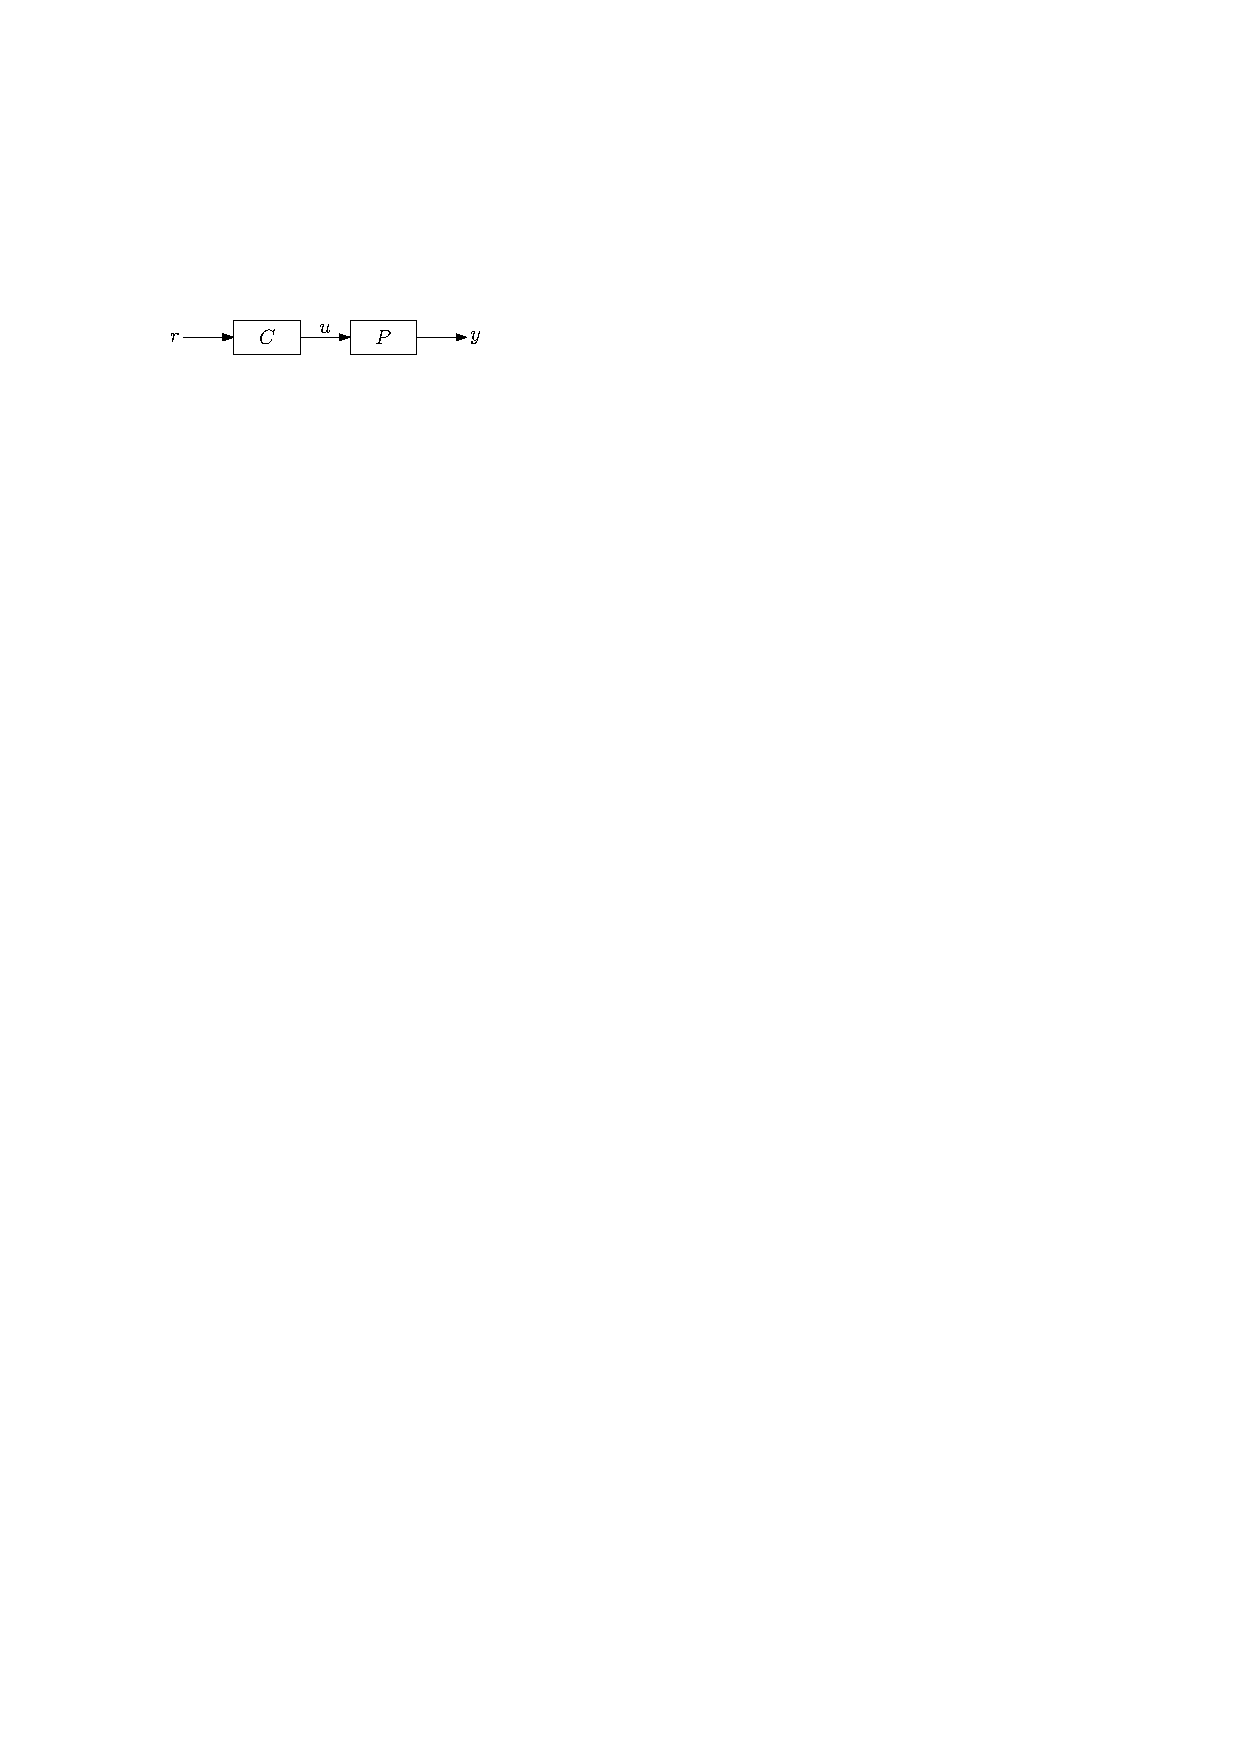
\includegraphics[width=0.5\hsize]{control/fig/block1.pdf}
\caption{最も単純なブロック線図の例. $C$はController (制御器) を, $P$はPlant (制御対象) を表している. }
\label{fig:block1}
\end{figure}
制御理論の詳しい内容には立ち入りませんが, 制御理論を用いて実装を行う際のポイントを軽く説明します. 
\par
\fig{block1}に最も単純なブロック線図の例を示します. 
このブロック線図においては, 何らかの指令値$r$を基にして制御器$C$が計算をして制御入力$u$を求めます. その後, 制御対象$P$に$u$を入力した結果, 出力$y$が観測される, という流れです. 
このように, 制御分野においては信号の流れをブロック線図という形で図示することでどのような処理を行っているかをわかりやすくするのが慣例です. 
\par
\begin{figure}[t]
\centering
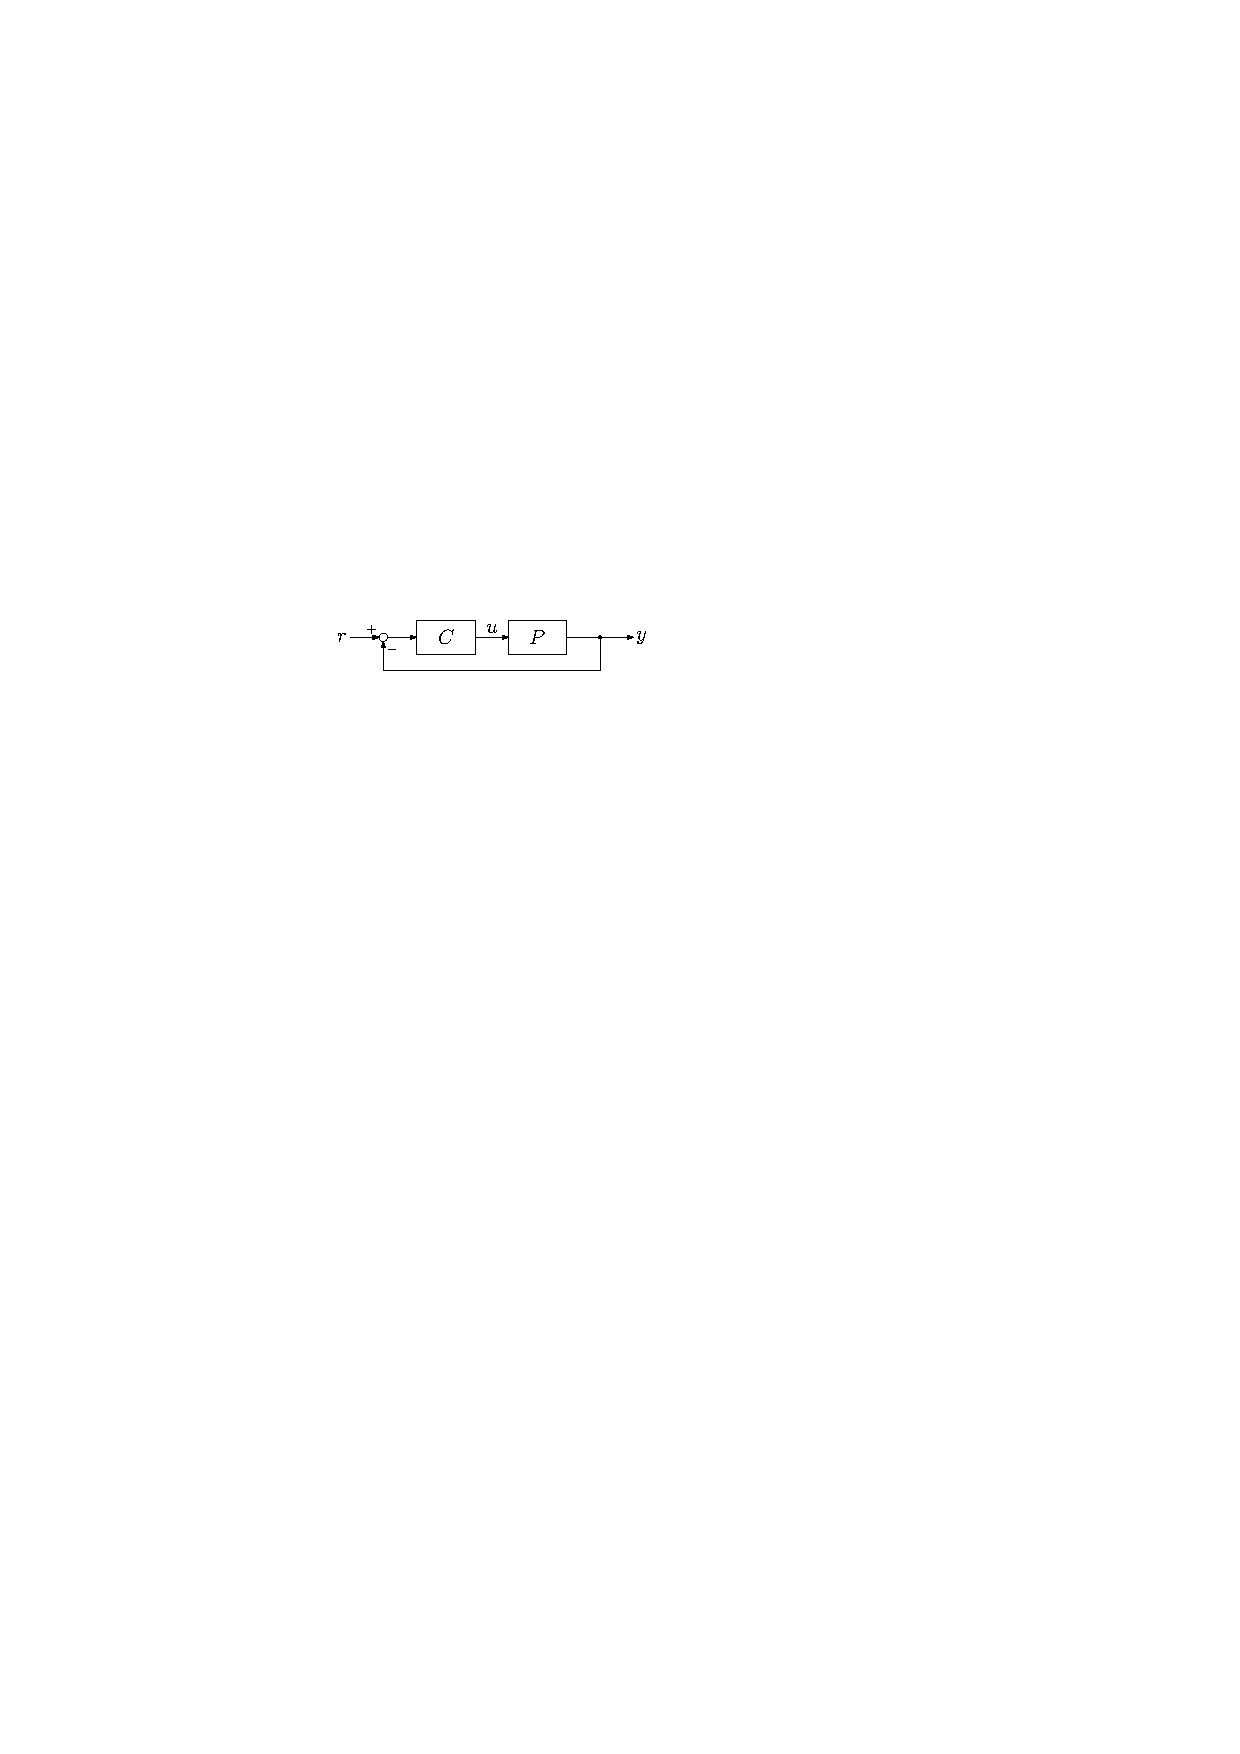
\includegraphics[width=0.5\hsize]{control/fig/block2.pdf}
\caption{\fig{block1}を少し複雑にしたブロック線図の例. }
\label{fig:block2}
\end{figure}
これを少しだけ複雑にしたものが\fig{block2}となります. 
\fig{block1}においては信号が左から右に進むだけだったのが, \fig{block2}では右から左への流れができています. 
このように, 信号が逆向きに戻っているような制御器のことをフィードバック制御器と呼びます. 
一方, 先程のように信号が一方向にのみ進んでいるような制御器のことはフィードフォワード制御器と呼びます. 
フィードフォワード制御では予めたてたPlantのモデル (例えば電流を入力するとモータトルクが発生し, それにより加速度がこの程度出るといった物理モデル) に基づき制御入力を計算します. 
したがって, この方法のみではモデルに含まれないような外乱がのった場合などに対処ができません. 
そこでフィードバック制御器を用いるとこの外乱により生じた$y$のずれを戻し, $r$から引くことにより, 適切な$C$のもとで$y$を$r$に近づけることが可能となります. 
ただし, この方法を用いるには何らかのセンサを用いて$y$を計測または推定する必要があることに注意してください. 
\par
\begin{figure}[t]
\centering
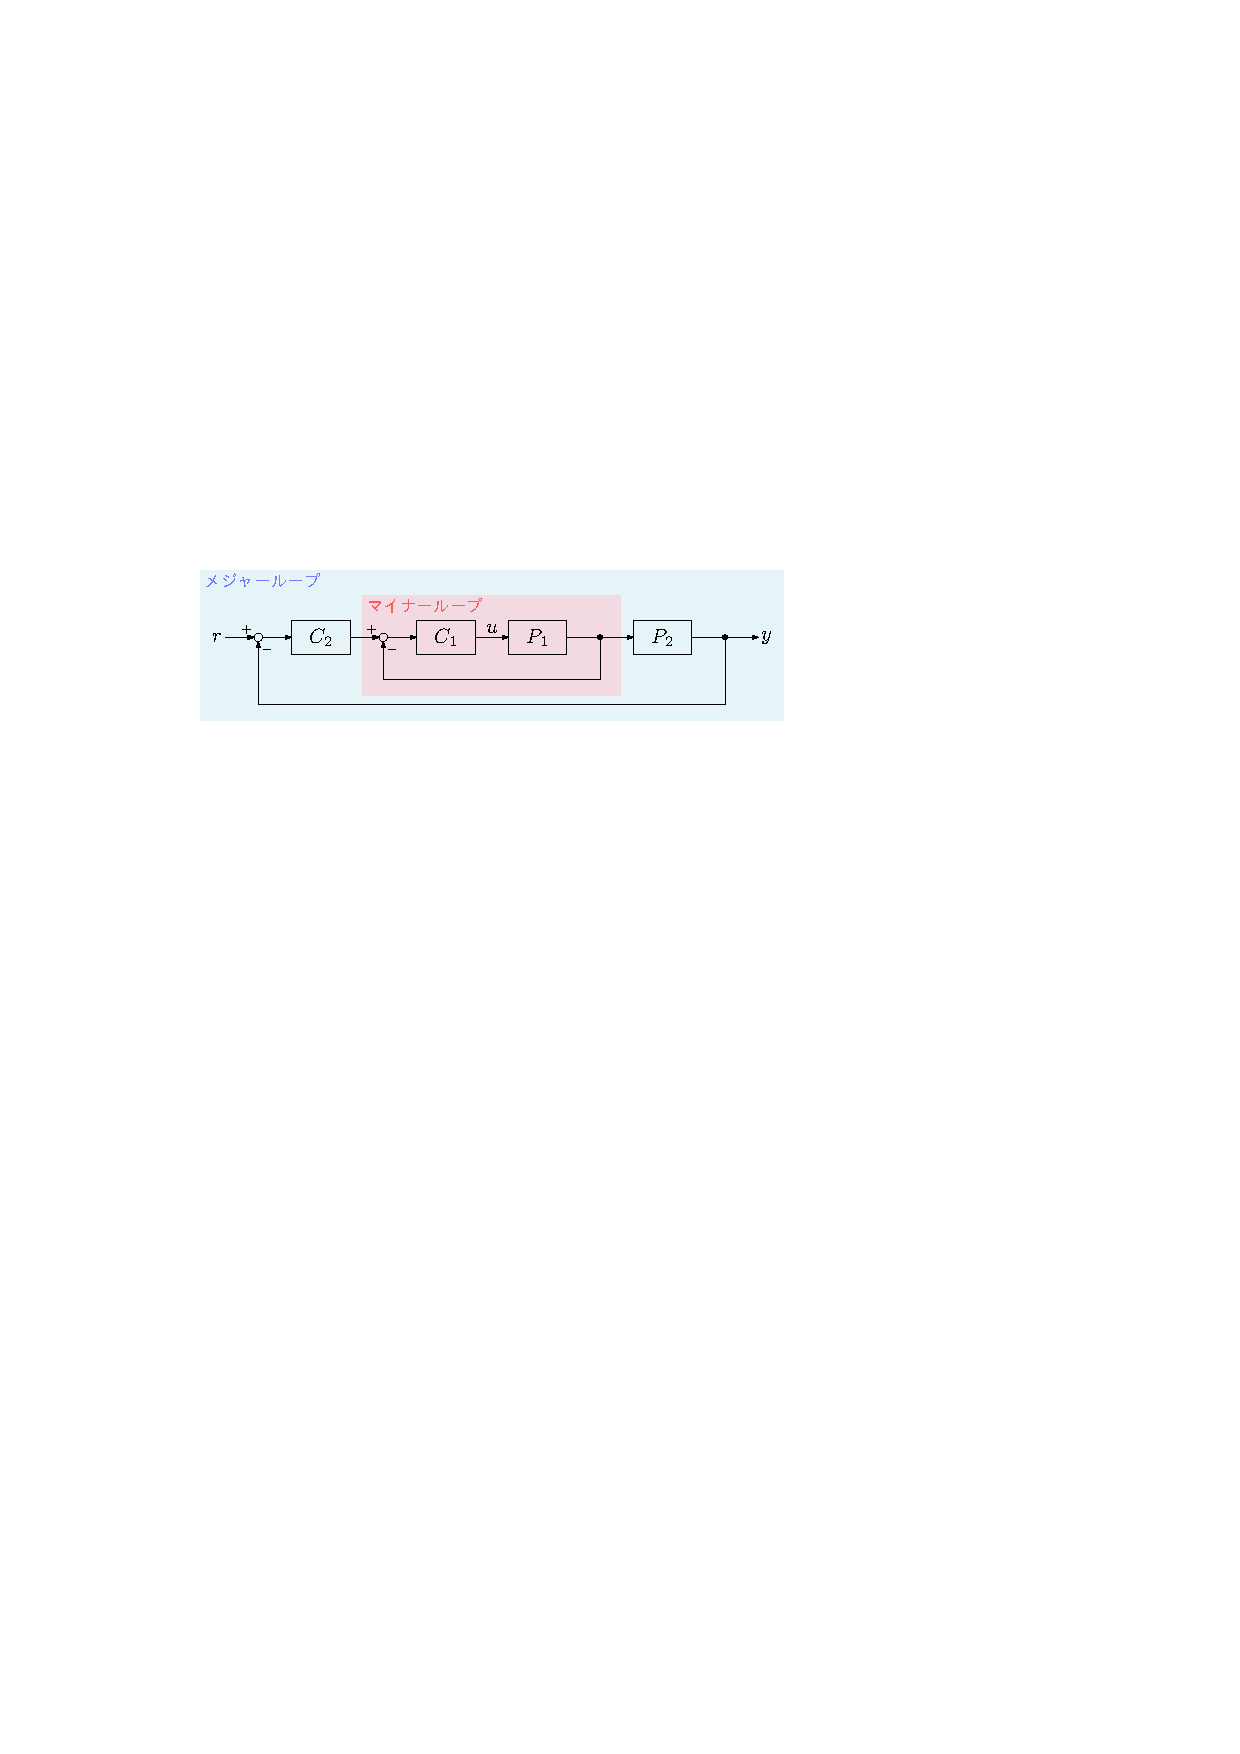
\includegraphics[width=0.8\hsize]{control/fig/block3.pdf}
\caption{二重にフィードバック制御器を組んだ場合のブロック線図の例. }
\label{fig:block3}
\end{figure}
先程のフィードバック制御系を二重にしたものが\fig{block3}です. 
一見するととてもややこしいように思えますが, 実際は先程のフィードバック制御器が2つあるだけに過ぎません. 
内側の$C_1$と$P_1$からなるループはマイナーループと呼ばれます. 
逆に外側の$C_2$と$P_2$からなるループはメジャーループと呼ばれます. 
これらは独立して考えることができ, マイナーループはメジャーループを単なる指令値を生成するブラックボックスとして扱うことができますし, 同様にメジャーループはマイナーループの実装については考える必要がありません. 
\par
これのわかりやすい例としてはメジャーループを速度制御系, マイナーループを加速度制御系としたものが挙げられます. 
メジャーループの速度制御器$C_2$により目標速度$r$と現在速度$y$から目標加速度が計算され, マイナーループの加速度制御器$C_1$によりモータ$P_1$に入力する電流$u$が求まります.  
もちろんこの場合, 速度制御系の更に外側に位置制御系が組まれることも考えられ, フィードバックループが何重にもなることもあります. 
その場合でもこのように各ループが綺麗に分かれていた場合は, それぞれをブラックボックスとして扱うことが可能です. 
\par
これは実際にロボットのプログラムに落とし込む際にとても大きなメリットを発揮します. 
各ループを独立に考えることが可能なため, 各ループに対応したレイヤー構成にすることでプログラムを綺麗に書くことが可能になります. 
すなわち, 位置司令値から速度指令値を求めるレイヤー, 速度指令値から加速度指令値を求めるレイヤー, 加速度指令値から電流指令値を求めるレイヤーなどに分割することでプログラムがわかりやすくなります. 
そもそも小さいプログラムだとレイヤー分けという概念自体あまり馴染みのないものかもしれません. 
しかし, 大きなプログラムを複数人で書くとなると適切にレイヤーを分け, レイヤー内のモジュール設計を適切に行うことが (ある意味実装よりも) 重要となります. 
このレイヤーの概念は先程のマイナーループ, メジャーループの考えとほぼ一致するものですが, レイヤーのパターン設計については様々な流派があることに注意してください. 
\par
最後に離散化について触れます. 
これまでブロック線図で見てきた信号の流れはすべて連続信号のように扱ってきました. 
しかしコンピュータが扱うのは離散化された信号であり, 一定周期ごとにサンプリングをして制御入力を決定することになります. 
この場合, 制御器を何らかの方法で離散化する必要が生じます. 
そのための手法として最も単純なものがゼロ次ホールド (ZOH) によるサンプリング・ホールドです. 
これは次の制御周期まで一定の入力をし続ける手法です. 
このような離散制御器による制御理論はディジタル制御として, 一般のシステム制御理論とは異なる体系となっているので, 興味がある人はそのような教科書や論文も読んでみてください. 
\section{センシングとモータ制御}
制御理論では可観測性と可制御性と呼ばれる指標があります. これは平たく述べると, センサを用いて状態を適切に推定できるか, またアクチュエータを用いて対象を適切に制御できるかということを表します. これらの具体的な求め方については割愛しますが, 推定・制御を適切に行うためにはセンサとアクチュエータを適切に配置する必要があることに注意してください. 
\par
以下ではそのセンサとアクチュエータについて実例をいくつか列挙します. 
\subsection{センサ}
ここではセンサの中でも特にロボットの自己位置を測定・推定するためのものに注目して述べます. 
\subsubsection{自己位置推定の種類}
\begin{itemize}
    \item デッドレコニング
    \par
    内界センサと呼ばれるセンサで得られる, ロボット自身の状態量の情報をもとにして自己位置を推定する手法です. 
    分解能が高く, 処理も比較的簡単ですが, 観測ノイズなどにより誤差が積算しやすいという問題があります. 
    \item スターレコニング
    \par
    外界センサと呼ばれるセンサで得られる, ロボット自身ではなく周囲の環境の情報をもとにして自己位置を推定する手法です. 
    デッドレコニングとは反対に, 誤差が積算することはありませんが, 処理が比較的重くなってしまいます. また分解能もデッドレコニングに比べると低くなる傾向があります. 
\end{itemize}
\subsubsection{内界センサの例}
\begin{itemize}
    \item ロータリーエンコーダ
    \par
    ロータリーエンコーダにも大きく分けて光学式と磁気式の2種類がありますが, どちらも回転角度を計測できるセンサです. 
    モータや車輪の回転数をロータリーエンコーダで測定し, 制御に用いることも多々ありますが, 自己位置推定目的では回転数計測専用の車輪にロータリーエンコーダを取り付けることが多いです. 
    これは, 駆動輪は摩擦力が足りずに滑ってしまうことがあり, その場合に正しくロボットの位置を測れなくなってしまうためです. 
    回転数計測用車輪とロータリーエンコーダを組み合わせることでロボットの移動距離を測定することができます. 
    
    \item 慣性センサ
    \par
    ジャイロセンサと加速度センサをまとめて慣性センサと呼びます. ジャイロセンサは角速度を, 加速度センサは加速度を, 直接得ることができます. これらの慣性センサのみでも3次元の姿勢・位置を推定することは可能で, 実際に航空機などでも慣性航法装置 (IMU) として使用されています. しかし, これらの観測値にはノイズが載ってしまうため, ロボコンにおいて慣性センサのみで自己位置を推定することは現実的ではありません. \par
    そこで, 先程のロータリーエンコーダ2つとジャイロセンサによりデッドレコニングを行う手法がよく用いられます. 
\end{itemize}
\subsubsection{外界センサの例}
\begin{itemize}
    \item 測距センサ
    \par
    超音波や光などを発し, その反射を受信することによって距離を測ります. 
    光源の種類や受信した信号から距離を算出する方法 (ToFと呼ばれる時間を用いるものや三角測量を用いるものなどがあります) の違いはありますが, どれも照射した方向までの距離が分かるのであまりロボットが回転しない競技などではとても強力なほか, デッドレコニングの補正用にも使用できます. 
    ただし, 取り付け角度の影響を受けやすい点には注意が必要です. 特にある程度遠くを測定したい場合には少しの設置角度のずれがとても大きな差になりかねません. 
    \item 測域センサ (LRF, LiDAR, レーザスキャナ)
    \par
    測距センサが1点のみの距離を測るものであったのに対し, 測域センサは2次元平面上の物体までの角度と距離を測ることが可能です. 
    一度に点群が得られる点は非常に強力ですが, 注意する点もあります. 
    \par
    まずひとつ目は点群の情報を処理することの大変さです. 点群とフィールドの情報からロボットの位置を推定する必要があり, その処理をするには制御担当のタスクも簡単ではありませんし, コンピュータにとっても比較的重い処理となります. 
    したがって, 測域センサを用いるにはマイコンではなく, シングルボードコンピュータまたはPCを使うことになります. 
    \par
    また, 測域センサのデータ取得周期が数十\si{\milli\second}と比較的遅いことも考慮に入れる必要があります. 
    ロボットが低速で動いているうちは大丈夫ですが, ある程度高速になると測域センサだけで自己位置を推定することは困難です. 
    その場合にはデッドレコニングと組み合わせるなどする必要が生じます. 
    
    \item ラインセンサ
    \par
    発光部と受光部があり, フィールドの色や明るさを読むことで自己位置を推定します. 
    測域センサよりは処理は軽くなることが多いですが, 内界センサや測距センサとは異なり, 計測値を処理する必要はあります. 
    また, 大会会場の照明やフィールドの色の違い・汚れなどの影響を受けやすいことも考慮しなければなりません. 
    \item カメラ
    \par
    画像処理を用いることでも自己位置推定を行うことができ, ビジュアルオドメトリと称されます. 
    画像処理も比較的重い処理なため, マイコンでの処理には向きません. 
    また, カメラも大会会場の照明の影響を受けやすい性質があります. 
\end{itemize}
\subsection{モータ}
\subsubsection{モータの種類}
ロボコンにおいてはバッテリーが電源として用いられるため, ロボコンにおいては普通DCモータが使われます. 
DCモータにも大別してブラシモータとブラシレスモータの2つがあり, それぞれ以下のような特徴を持ちます. 
\begin{itemize}
    \item ブラシモータ\par
    ブラシモータは高校の電磁気などでも出てくるようなブラシと整流子が接触し, コイルに電流が流れることにより回転トルクが発生するようなモータです. 
    電圧を印加するだけで回転するため動作させるのが簡単でかつ構造も簡単なため安価で購入できるというメリットがあります. 
    一方で, ブラシの接触によりノイズが発生するほか, ブラシの摩耗により性能は次第に劣化していきます. 
    
    \item ブラシレスモータ\par
    ブラシレスモータはブラシモータと違ってブラシと整流子が存在せず, 電子制御により電流の向きを変えることで回転トルクを発生させます. 
    ブラシモータの欠点であったブラシを持たないため, ノイズの少なさや効率・制御性の良さなどの利点を持ちます. 
    一方でタイミングよく電流の向きを切り替える必要があることから, センサによる測定や推定を行った上で制御する必要があり, 必要な回路も異なることため, ブラシモータと比べると動作させるためのコストは大きくなります. 
\end{itemize}
\subsubsection{モータのスペック}
モータを選定するためにはモータスペックの見方について知る必要があります. 
以下に主要なものを挙げますが, メーカによっては公表されていないものもあることに注意してください. 
\begin{itemize}
    \item トルク定数 [\si{\newton\metre/\ampere}]: トルクは電流に比例するが, その比例定数
    \item 最大連続電流 [\si{\ampere}]: 連続して流し続けられる電流の最大値
    \item 無負荷時回転数 [\si{\radian/\second}]: 定格電圧印加時にモータに負荷をかけないときの回転数
    \item 停動トルク [\si{\newton\metre}]: 定格電圧印加時に回転速度が0となるときのトルク
    \item 端子間抵抗 [\si{\ohm}]: モータの持つ内部抵抗
    \item KV値: 主にブラシレスモータでよく用いられる値で\SI{1}{\volt}上昇したときに回転数がどれだけ上がるかを表した値
    \item 最大効率
\end{itemize}
\par
これらのスペックをもとにして, モータの選定を行います. 
モータを選定する際に必要なこととして, まず必要な速度とトルクを見積もることがあります. 
これは足回りであればどれくらいの重量のロボットをどれくらいの加速度・最高速度で動かしたいのか, アームなどであればどの程度のオブジェクトを掴むものをどれくらいの加速度・最高速度で動かしたいのかを決めることで, 力学計算により求めることができます. 
\par
次にその必要なトルク・速度要求を満たすモータを選んでいきます. 
まず, トルク定数と最大連続電流から最大トルクが計算できます. 
瞬間的であればこの値を超えてトルクを出すこともできますが, 連続して出し続けるとモータが熱で焼ける恐れがあります. 
また, 横軸にトルク, 縦軸に回転数を取り, 無負荷時回転数と停動トルクの2点を結ぶ直線を引くと, \fig{motor}のようにトルクと回転数の関係が表せます. 
これは回転数を上げるとトルクが出せず, 逆にトルクを出すと回転数が上げられないことを意味します. 
これらより最大トルクでの回転数も算出できます. 
この2つがともに要求値を超えていれば, 要求を満たしていることになります. 
\par
ここまで考えていたのは減速機を挟まない場合でした. 
しかし, 速度とトルクのバランスが望み通りのモータが見つかる場合はごくまれです. 
そこで減速機を用いることでよりトルク寄りにしたり速度寄りにして, モータの出力が要求を満たすような減速比を選ぶことが重要になります. 
ただし, 減速機の伝達効率によりトルクに損失が生じてしまう点や, 減速機自体のトルク・回転数定格も上回ってはいけない点に注意する必要があります. 
\begin{figure}[t]
    \centering
    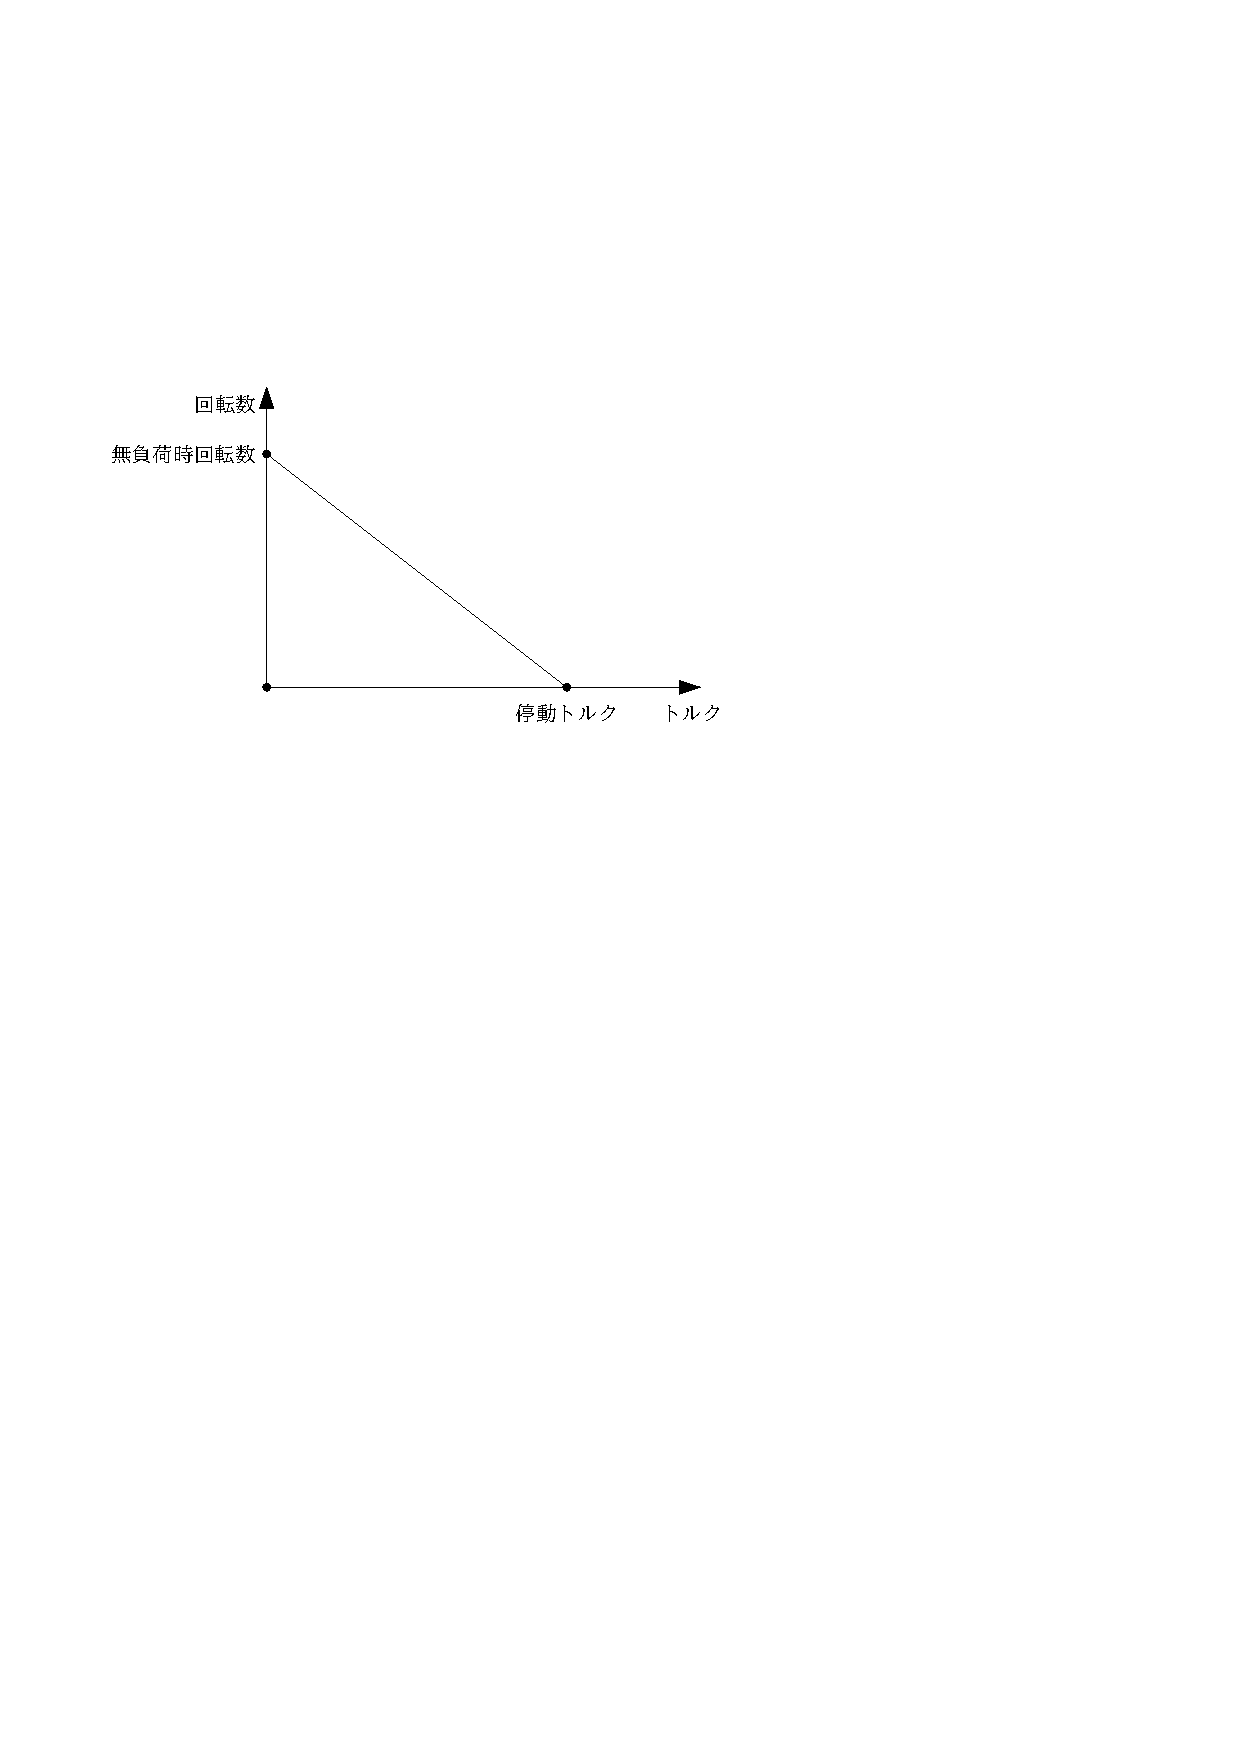
\includegraphics[width=0.5\hsize]{control/fig/motor.pdf}
    \caption{モータの特性を表すトルク-回転数グラフの概略.}
    \label{fig:motor}
\end{figure}

%こっから下は消すか迷い中
\section{その他}
\subsection{チーム開発}
チーム開発は個人開発と違った難しさが存在します. 
その解決策として以下の3つを行うことをおすすめします. 
\begin{enumerate}
    \item 標準環境を決める
    \par
    人によってOSやコンパイラ, ライブラリなどのバージョンが違うと, 同じソースコードなのにビルドできる人とできない人が出てくるなど, トラブルのもととなります. 
    そこで, 標準の環境を決めておき, それぞれがそれに準拠した環境を用意するのがおすすめです. 
    ロボットにPCを搭載する場合は, それも可能な限り手元と同じ環境にしておくと良いでしょう. 
    \item バージョン管理ツールを使う
    \par
    Gitに代表されるようなバージョン管理ツールを使ってソースコードを管理することをおすすめします. 
    このようなツールを用いることで, 複数人が別々に編集したものを容易に合体できるほか, ある変更を加えて動作がおかしくなったときでも, うまく動いていたときのソースコードに戻すことが可能になります. 
    \item コードレビューをする
    \par
    身をもって経験したことのある方も多いかもしれませんが, プログラミングにバグはつきものです. 
    しかしコードレビューをすることによってバグを未然に防ぐことができるかもしれません. 
    またソースコードが属人化, つまり書いた本人しかわからないようになってしまうと, その人がいないと改修できないなど開発効率が低下してしまいます. 
    このような事態も, コードレビューを行うことにより他人の書いたコードを把握することで防ぐことが可能です. 
\end{enumerate}
\subsection{論文のすすめ}
ロボコンで用いる技術の中には, 制御工学やロボティクスの分野においてすでに定式化され解決されているものも多く存在します. 
書籍, とくに和書はなかなか最新の情報や専門的な情報が得られにくく, インターネット上の情報は玉石混交な上にこちらも専門的なものは多くありません. 
そこで, そのような専門的な情報であっても容易に手に入れられ, 比較的信頼できるのが論文です\footnote{査読という審査を経て公開されているものであれば一定の信頼はおけますが, 全幅の信頼をおくことはせずに疑ってかかることは不可欠です}. 
自ら考えることも重要ですが, まずは似たような問題が解かれていないか論文を探してみることをおすすめします. 
\par
探し方は各校でも紹介されていると思いますが, Google ScholarやIEEE Xplore, Science Directなどを使ってみると良いでしょう. 
%\subsection{コンピュータ}
%計算機を知ろう
%\subsection{プログラミング}
%はやいのとおそいの
%